\chapter{Configuração do NAT} \label{nat}

\textbf{NAT} (Network Address Translation) é um protocolo de atribuição de endereços IP público não atribuídos para acesso à Internet \cite{nat}.
Permite a conservação do endereços IP, de modo a garantir que não há endereços IP reservados a não ser utilizados, dado que há um número finito de endereços disponíveis.

Na estrutura de rede considerada, apenas a DMZ tem acesso à internet.
Deste modo, apenas temos que configurar o NAT para as interfaces usadas pela DMZ.

\begin{figure}[H]
    \centering
    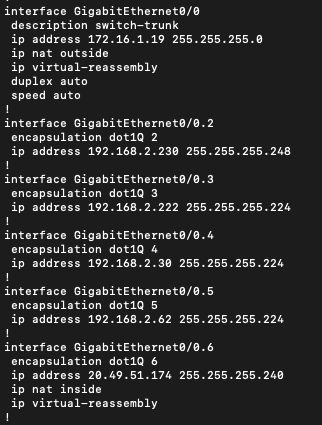
\includegraphics[width=.65\linewidth]{figs/nat/nat_router.png}
    \caption{Configuração do NAT nas interfaces GE0/0 e GE0/0.6}
    \label{fig:nat_router}
\end{figure}

Para configurar o NAT, é sempre preciso definir uma interface \textit{NAT inside} e outra \textit{NAT outside}.

A interface \textbf{NAT Inside} corresponde à origem do tráfego interno que tem como destino a internet.
Neste caso, o tráfego provém apenas da DMZ, pelo que apenas a sua interface foi configurada (GE0/0.6)

A interface \textbf{NAT Outside} corresponde à interface que tem ligação ao exterior, isto é, à internet.
Neste caso, a interface é que se tem que definir é aquela que está ligada ao \textit{Firetux} (GE0/0).

Para testar se o NAT foi bem configurado, fazemos um \textit{ping} a um endereço externo, como por exemplo \verb|google.com|.

\begin{figure}[H]
    \centering
    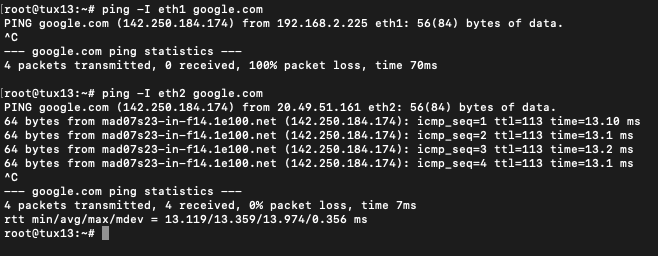
\includegraphics[width=.8\linewidth]{figs/nat/nat_ping.png}
    \caption{Ping nas interfaces eth1 e eth2}
    \label{fig:nat_ping}
\end{figure}

Como se observa, a interface \textbf{eth1} que corresponde à rede de servidores, que não tem acesso à internet.
Com a interface \textbf{eth2} que corresponde à DMZ, o \textit{ping} é bem sucedido.
Nas restantes interfaces / sistemas, o \textit{ping} também não é bem sucedido como seria de esperar.

